Поскольку производительность системы mmWave зависит от точности формирования ДН,
основная задача этой работы заключается в разработке точного алгоритма оценки
АОА. Рассматриваемая задача имеет множество существенных ограничений, которые
учитываются в этом исследовании.  Во-первых, разработанный алгоритм должен быть
основан на пилотных сигналах стандарта 5G NR, то есть он должен иметь
фиксированную дискретную временн\'{у}ю структуру. \hl{В качестве } Во-вторых,
алгоритм должен выполняться на стороне пользователя и БС не может изменять свою
схему прозвонки.  В-третьих, при смене центрального направления ДН возникают
скачки фазы, что требует дополнительных калибровок и затрудняет когерентный
прием сигнала, поэтому желательно, чтобы алгоритм был основан только на
измерениях мощности и не зависел от фазы сигнала.

На основе проведенного обзора литературы (см. \ref{sec:review}) мы выделили и
разработали несколько подходов, отвечающих вышеперечисленным требованиям. Первый
подход, в качестве базового алгоритма был выбран иерархический поиск (см.
\ref{sec:hierarchy:search}).  Это простейший метод, который адаптивно
аппроксимирует алгоритм Фурье (см. \ref{sec:fourier}).  Основной проблемой этого
алгоритма будет ошибка квантования.  В данной работе разработан новый алгоритм,
основанный на идее иерархического поиска.  Он использует улучшенную схему
измерения и получает оценку без ошибки квантования на основе критерия
минимума среднеквадратичной ошибки (MMSE).

Второй рассматриваемый алгоритм основан на моноимпульсе (см.
\ref{sec:monopulse}), идея которого была предложена в \cite{Zhu2016, Kim2019},
но только для одной антенной решетки. В данной работе этот алгоритм тестировался
и модифицировался под выбранную аппаратную конфигурацию.  Этот алгоритм также
обеспечивает непрерывный результат.

Третий рассмотренный алгоритм, так называемый \textit{Adaptive Compressed
Sensing Algorithm}, который был предложен в \cite{Alkhateeb2014}.  Этот алгоритм
представляет собой схему бинарного поиска со специальной кодовой книгой. Это
одно из самых простых и эффективных решений, среди подобных алгоритмов.  Кроме
того, он основан исключительно на мощностных характеристиках принятого сигнала.
Однако описанное решение и кодовая книга подойдут только для очень больших
антенных решеток со степенями свободы как по фазе, так и амплитуде. Для
выбранной конфигурации, описанное в \cite{Alkhateeb2014} нельзя применить
напрямую, поэтому алгоритм пришлось модицицировать.  Основным преимуществом
этого алгоритма по сравненю с остальными двумя является малое временя зондирования.

Все упомянутые выше алгоритмы были модицицированы для оценки многолучевого AOA.

В этом разделе приведено подробное описание алгоритмов, схем измерений. В
разделе \ref{sec:simulations} представлены результаты моделирования.


\subsection{Структура пилотных сигналов в системах 5G NR}
\label{sec:ssburst}

\hl{В данной работе используется }
Стандарт 5G NR включает два типа опорных сигналов, которые можно использовать для обучения луча: SS-burst
и CSI-RS.

SS-burst представляет собой специальный набор опорных сигналов -- блоков
синхронизации (SS blocks), предназначенных для первоначального доступа. Пилотные
сигналы занимают полосу в 127 поднесущих с шагом по частоте 125 кГц. 
Каждый блок синхронизации передается с уникальным весовым вектором, что 
позволяет за один SS блок прозвонить только одну пару лучей.  
Максимальное количество SS блоков в SS-burst равно 64. 
SS-burst повторяются с периодом, находящимся  в диапазоне от 5 до 160 мс \cite{Dahlman2018}.  
В работе выбрано значение 20 мс.

\begin{figure}[h!]
    \centering
    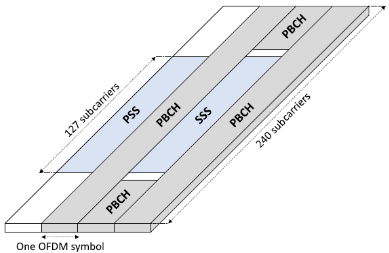
\includegraphics[width=0.4\linewidth]{figs/fig4.1}
    \caption{Структура блока синхронизации}
    \label{fig:4.1}
\end{figure}
\begin{figure}[h!]
    \centering
    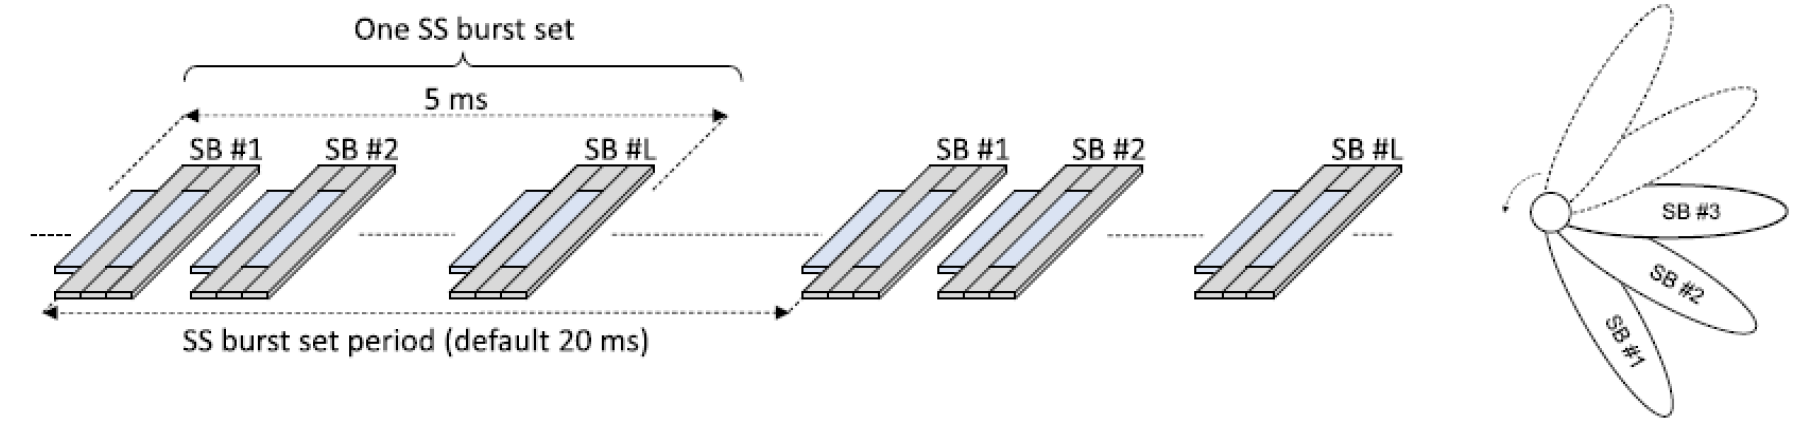
\includegraphics[width=\linewidth]{figs/fig4.2}
    \caption{Последовательность блоков синхронизации (SS-burst)}
    \label{fig:4.2}
\end{figure}

\subsection{Пользовательская система антенных решеток}

\begin{figure}[ht]
    \centering
    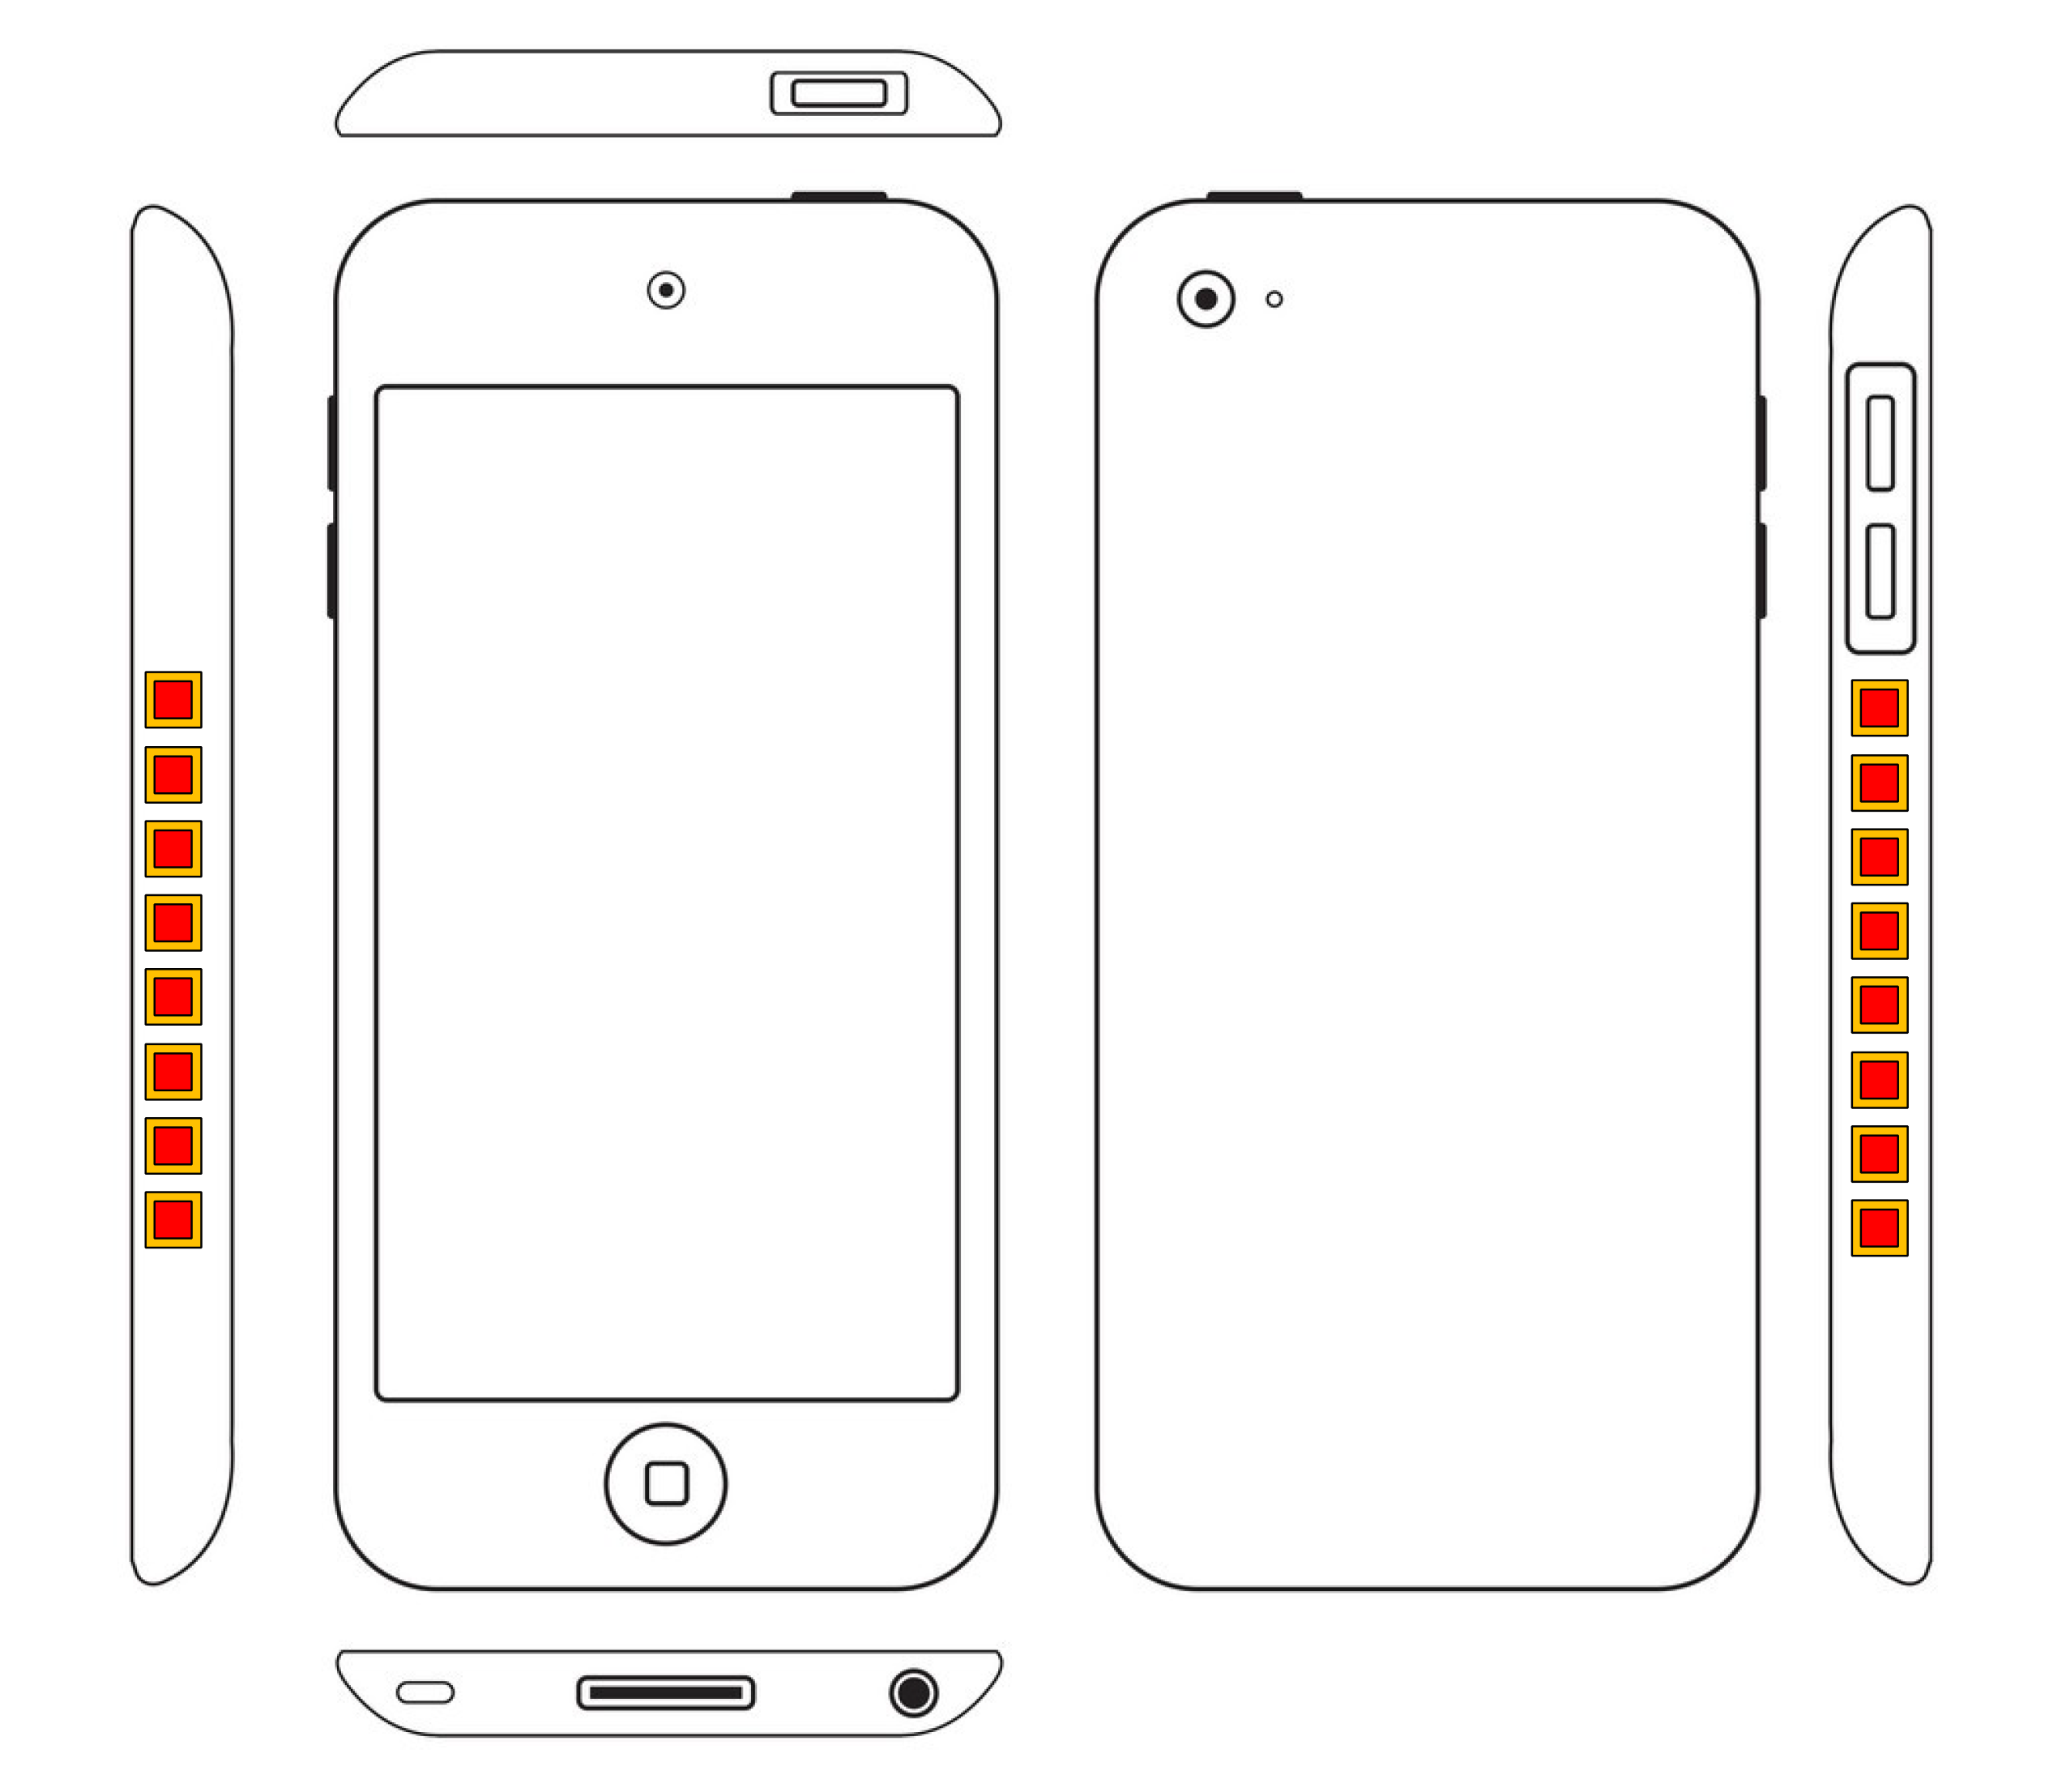
\includegraphics[width=0.5\linewidth]{figs/fig4.3}
    \caption{Расположение антенных решеток на мобильном устройстве}
    \label{fig:4.3}
\end{figure}

\begin{figure}[ht]
    \centering
    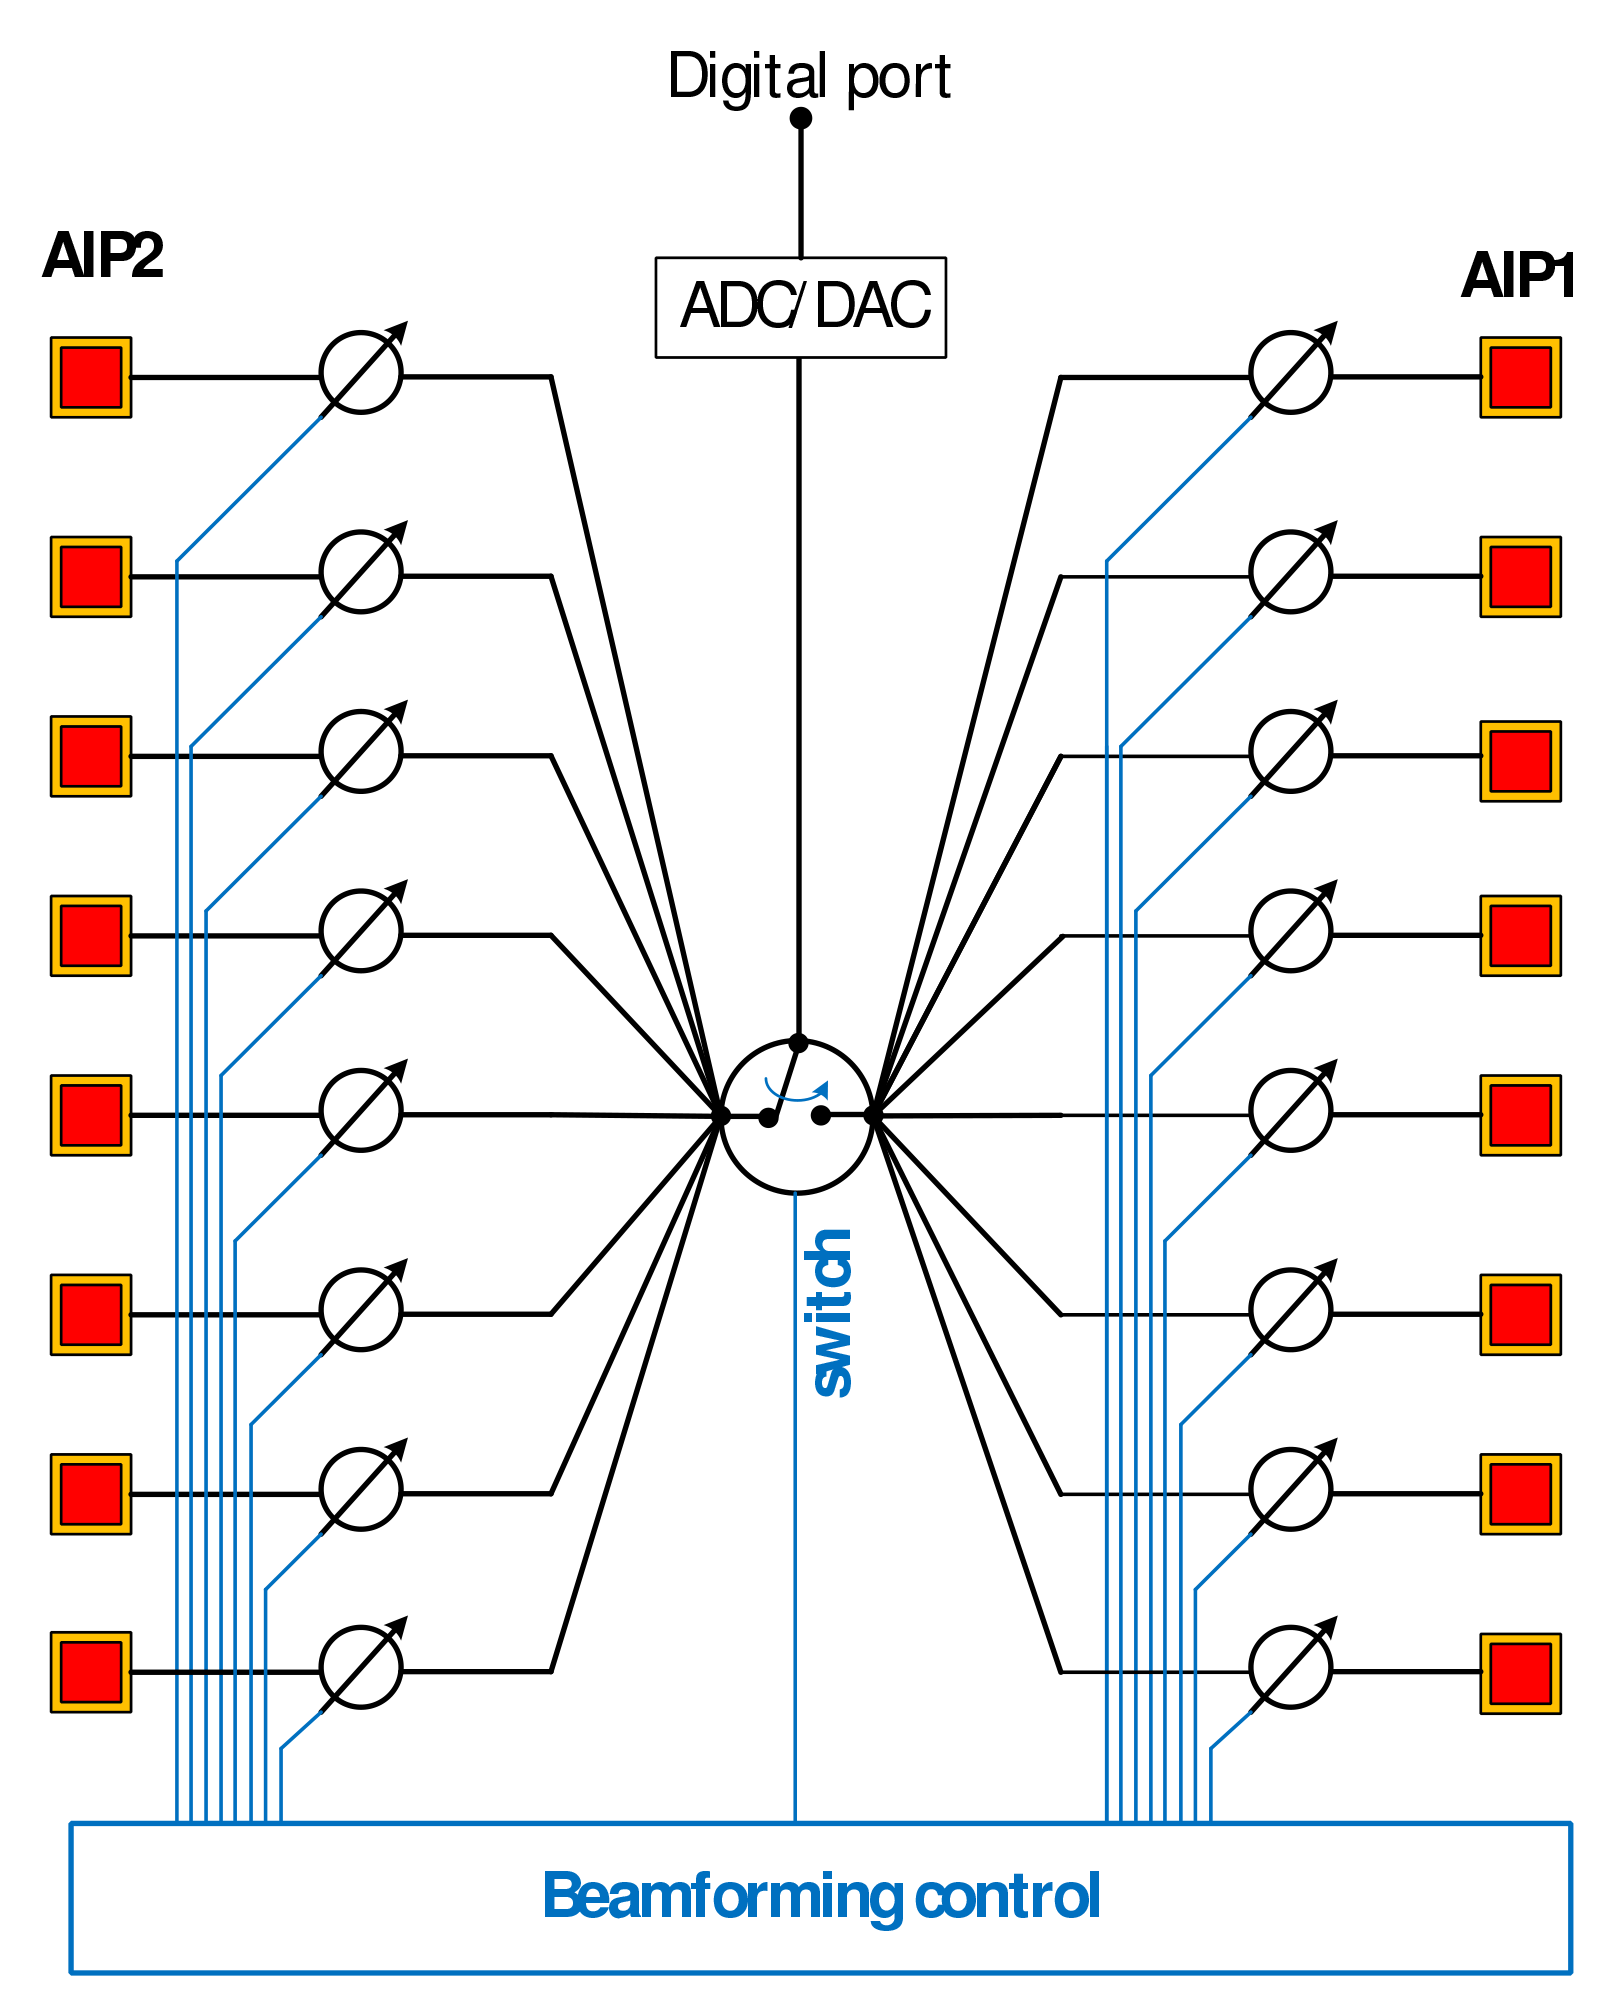
\includegraphics[width=0.4\linewidth]{figs/fig4.4}
    \caption{В системе присутствует только один АЦП и независимые фазовращатели для каждого элемента АР}
    \label{fig:4.4}
\end{figure}

В данной работе разрабатываются алгоритмы для системы, состоящей из двух линейных эквидистантных антенных решеток, расположенных на противоположных сторонах
устройства (см. \ref{fig:4.3}). В данной конфигурации оборудования, у пользователя нет слепых зон в азимутальной плоскости.

Система содержит только один цифровой порт (АЦП). Таким образом, решетки не могут
использоваться одновременно и возможно только переключение между ними.

Формирование ДН происходит с помощью непрерывных независимых аналоговых фазовращателями, как показано
на \ref{fig:4.4}.  Диаграмма направленности каждого антенного элемента устанавливается в
соответствии с таблицей 7.3-1 стандарта 3GPP TR 38.901. Ширина луча по уровню -3
дБ составляет $65^\circ$, усиление составляет 8 дБи, ослабление мощности, поляризация предполагается вертикальной.





Также стоит определить что подразумевается под угловой координатой источника
излучения.  Поскольку выбранная конфигурация АР линейна, невозможно одновременно
азимутальный угол и угол места принятого излучения.  Однако линейная решетка
может определить обобщенный угол $\psi$. Можно рассматривать некоторый
эффективный азимутальный угол $\phi_{eff}$ в качестве угловой координаты
источника, который удовлетворяет следующему уравнению
\begin{equation}
    \label{eq:4.1}
    \psi = 2\pi \frac{d}{\lambda} \sin \phi_{eff} = 2\pi \frac{d}{\lambda} \sin\phi \cos{\theta},
\end{equation}
\begin{equation}
    \label{eq:4.2}
    \phi_{eff} = \arcsin(\sin \phi \cos \theta),
\end{equation}
где $\phi$ и $\theta$ -- геометрические углы азимута и элевации источника.

\begin{figure}[ht]
    \centering
    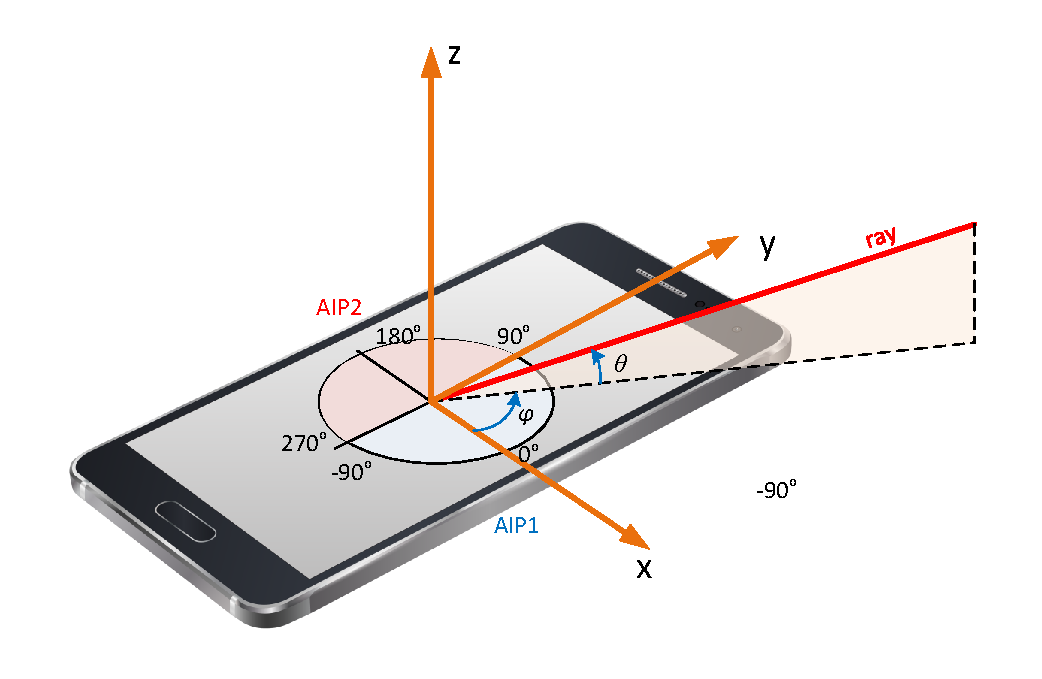
\includegraphics[width=0.75\linewidth]{figs/fig4.5}
    \caption{Локальная система координат пользователя}
    \label{fig:4.5}
\end{figure}

\subsection{Антенная решетка базовой станции и система прозвонки}

Антенная решетка базовой станции представляет собой эквидистантную плоскую
антенную решетку с 12 строками и 16 столбцами с двумя цифровыми портами.
Формирование диаграммы направленность происходит независимыми непрерывными
аналоговыми фазовращателями. Таким образом, можно одновременно прозвонить два
луча, если это позволяет структура пилотного сигнала.

Диаграмма направленности антенного элемента устанавливается в соответствии с
таблицей 7.3-1 стандарта 3GPP TR 38.901. Ширина луча элемента по уровню $-3$ дБ
составляет $65^\circ$. Усиление составляет 8 дБи, \hl{ослабление мощности с задней
стороны решетки составляет -30 дБ}, поляризация предполагается вертикальной.

В результате имеется 192 пары ортогональных лучей для этой антенной решетки.
Однако мы не сможем прозвонить их все за один SS-burst (см. \ref{sec:ssburst}),
поскольку нам доступно только 64 возможных прозвонки. Для решения этой проблемы
можно учесть две особенности.  Во-первых, пользователи в пространстве перемещаются больше в
горизонтальной плоскости, чем в вертикальной. Поэтому можно увеличить ширину
луча в вертикальной плоскости и уменьшить количество лучей с различными углами
элевации.  Во-вторых, в mmWave системе пользователи обычно располагаются ниже
БС, поэтому лучи соответствующие верхнему подпространству БС могут не
рассматриваться.

Тогда, проблема решается следующим образом:
\begin{itemize}
    \item Верхние 4 ряда антенной решетки БС отключаются (см. \ref{fig:4.6}), обеспечивая более широкую ДН в вертикальной плоскости
    \item Кодовая книга БС выбирается на основе метода Фурье (см.
    \ref{sec:fourier}). Горизонтальная сетка обобщенных углов $-\pi +
    pi/16:\pi/8:\pi-\pi/16$.
          Вертикальная сетка обобщенных углов $-3\pi/4:\pi/4:0$.
    \item Представленная кодовая книга покрывает нижнюю половину пространства (см. \ref{fig:4.6}), где, как ожидается, будет находиться пользователь.
\end{itemize}

\begin{figure}[ht]
    \centering
    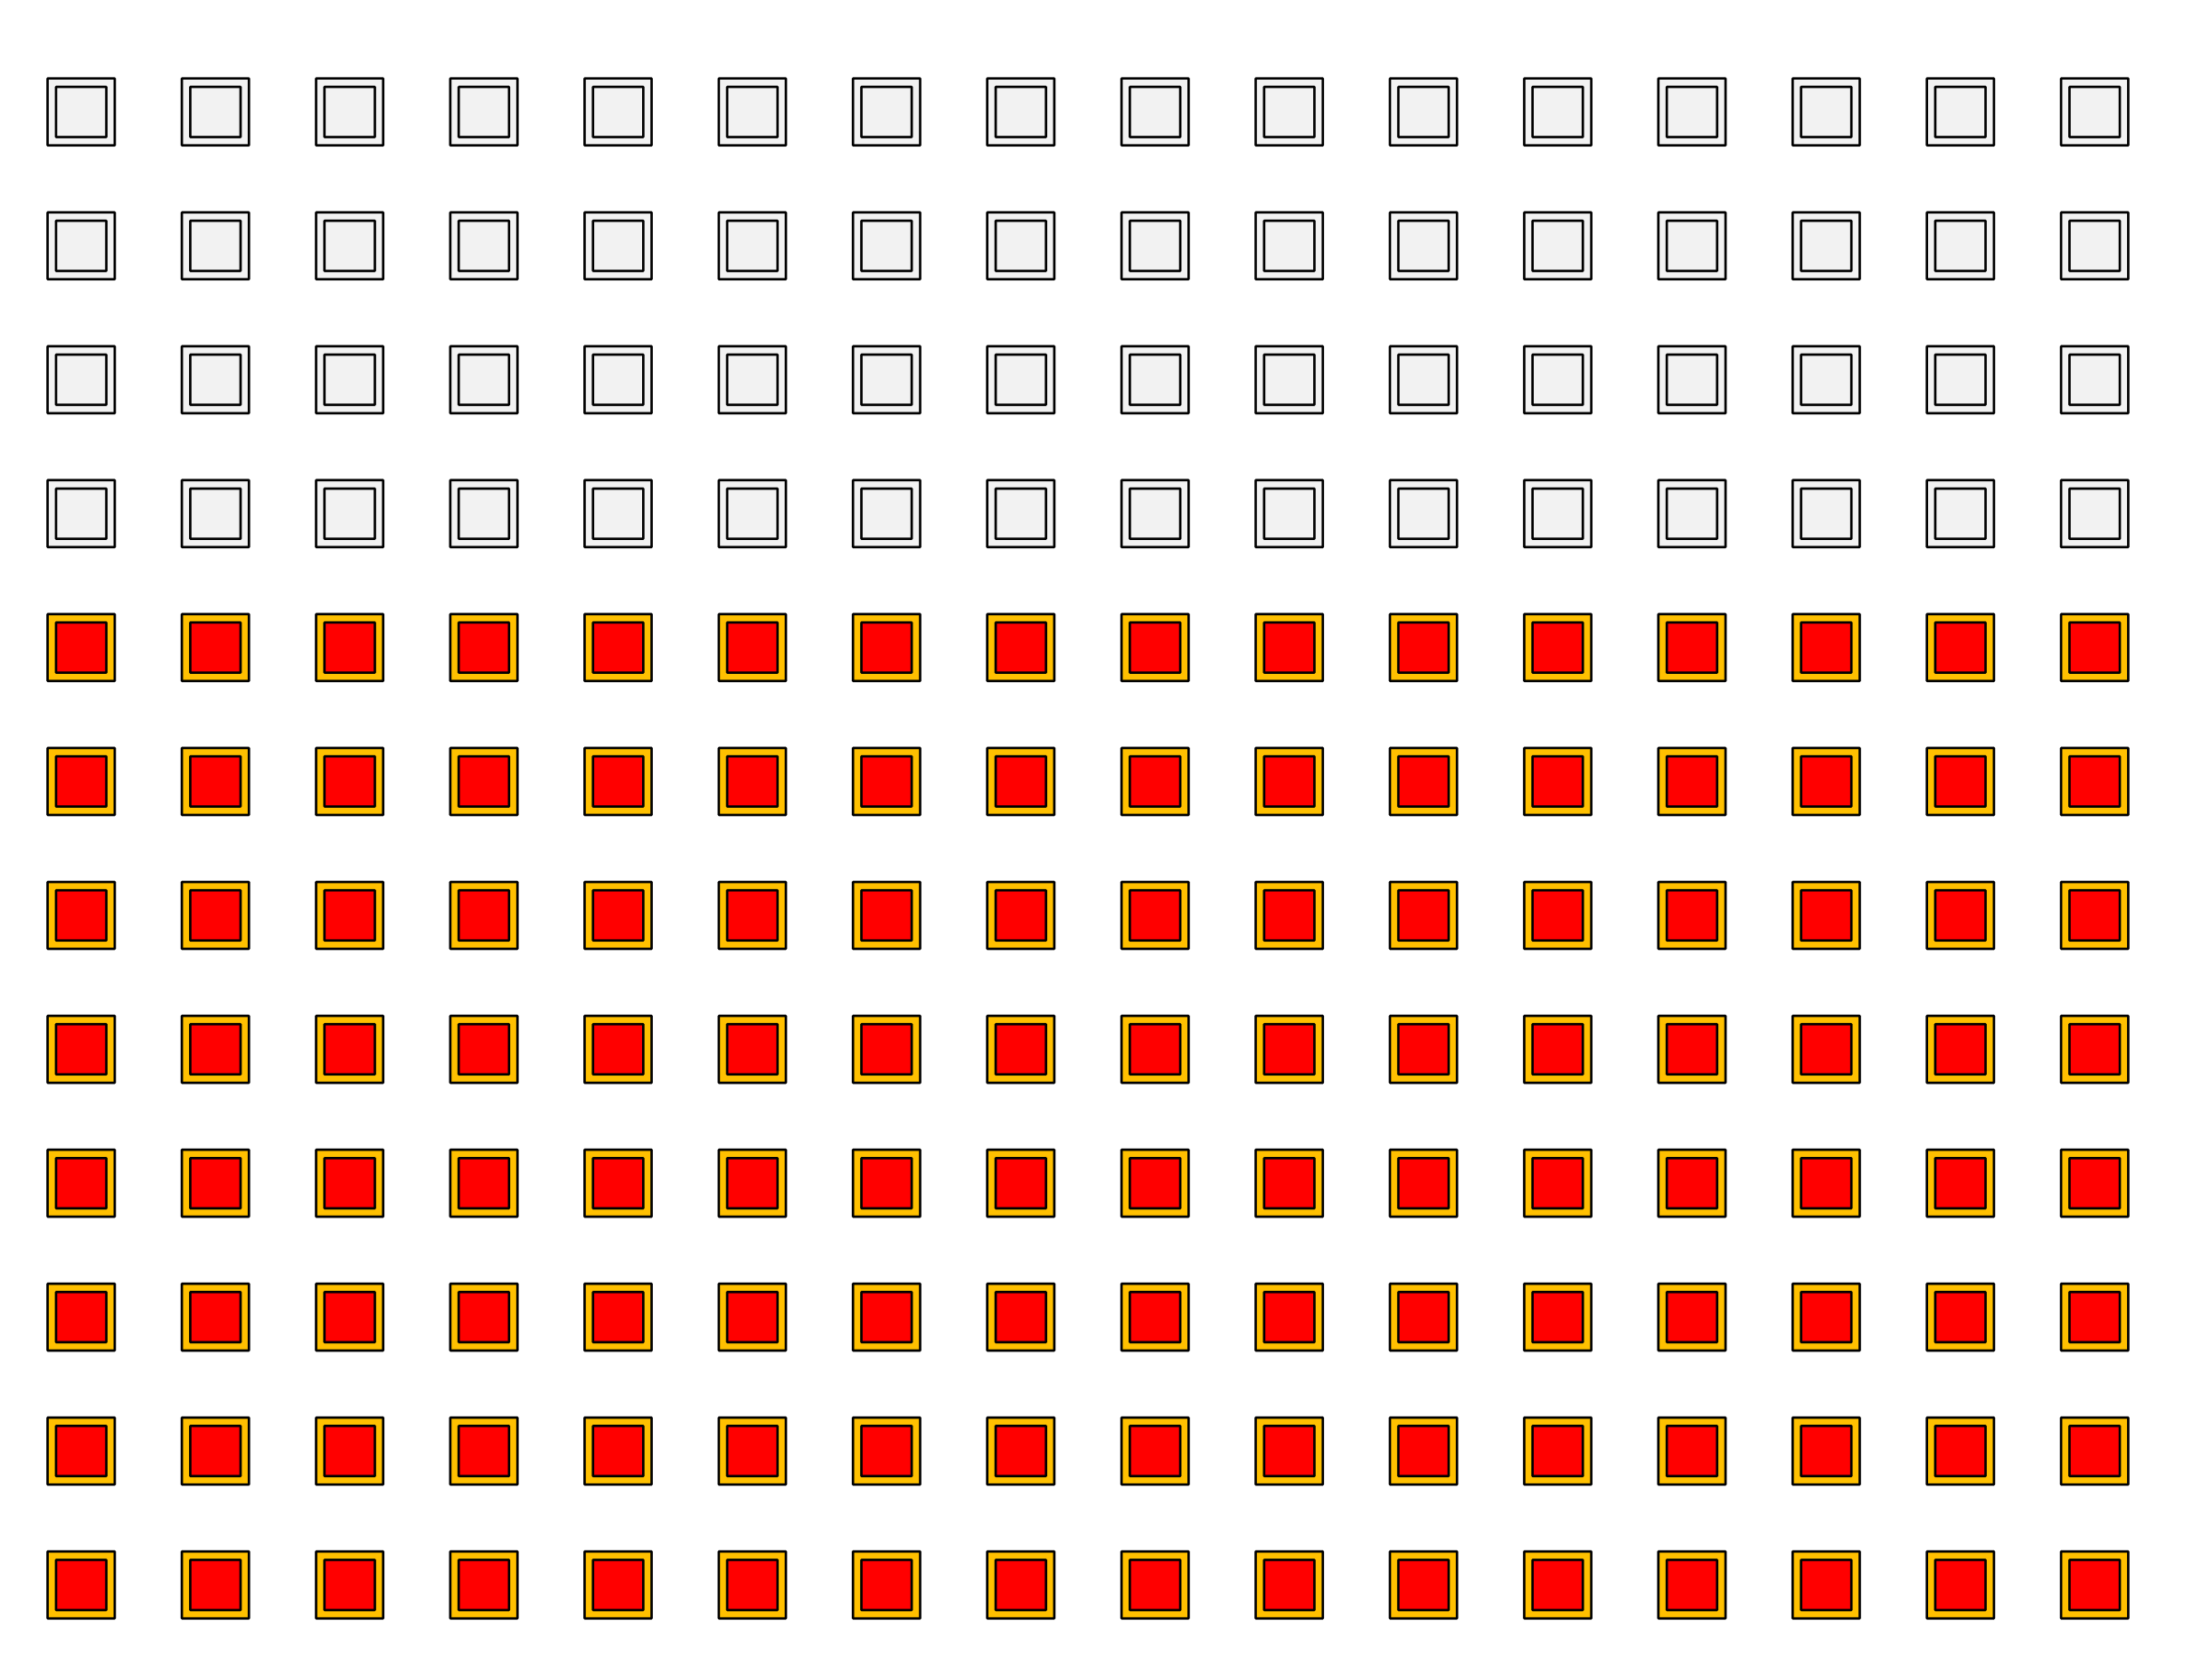
\includegraphics[width=0.35\linewidth]{figs/fig4.5.png}
    \caption{Серые элементы антенной решетки отключены во время оценки угла прихода}
    \label{fig:4.6}
\end{figure}

\begin{figure}[ht]
    \centering
    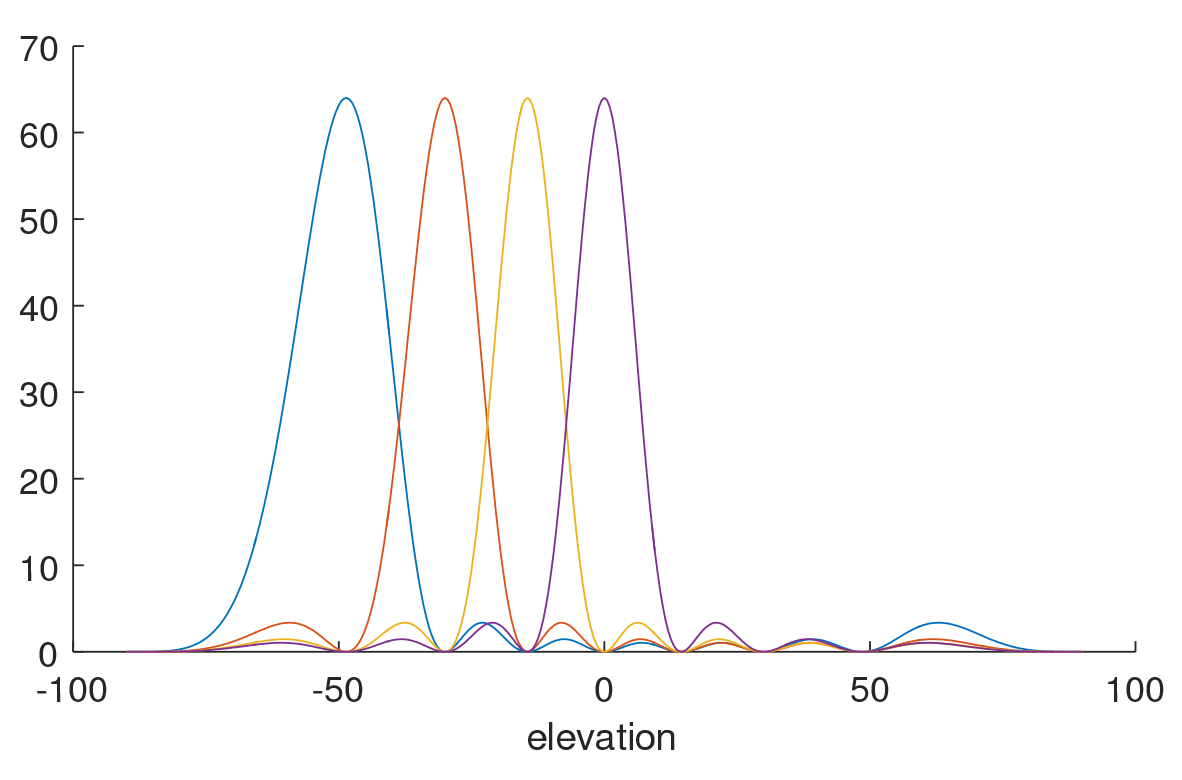
\includegraphics[width=0.5\linewidth]{figs/fig4.6}
    \caption{ДН антенной решетки БС в вертикальной плоскости}
    \label{fig:4.7}
\end{figure}


<<<<<<< HEAD
=======
CSI-RS рассматривается как наиболее предпочтительный сигнал для быстро меняющегося канала. 
Но чтобы уменьшить время зондирования, количество
зондируемых лучей БС должно быть значительно уменьшено. Предлагается
использовать 8 ортогональных лучей в горизонтальной плоскости с квази изотропным распределением 
в вертикальной плоскости.
Чтобы реализовать эту схему формирования луча, необходимо отключить все
элементы, кроме первой половины первой строки (см. рис. \ref{fig:4.8}).

\begin{figure}[ht]
    \centering
    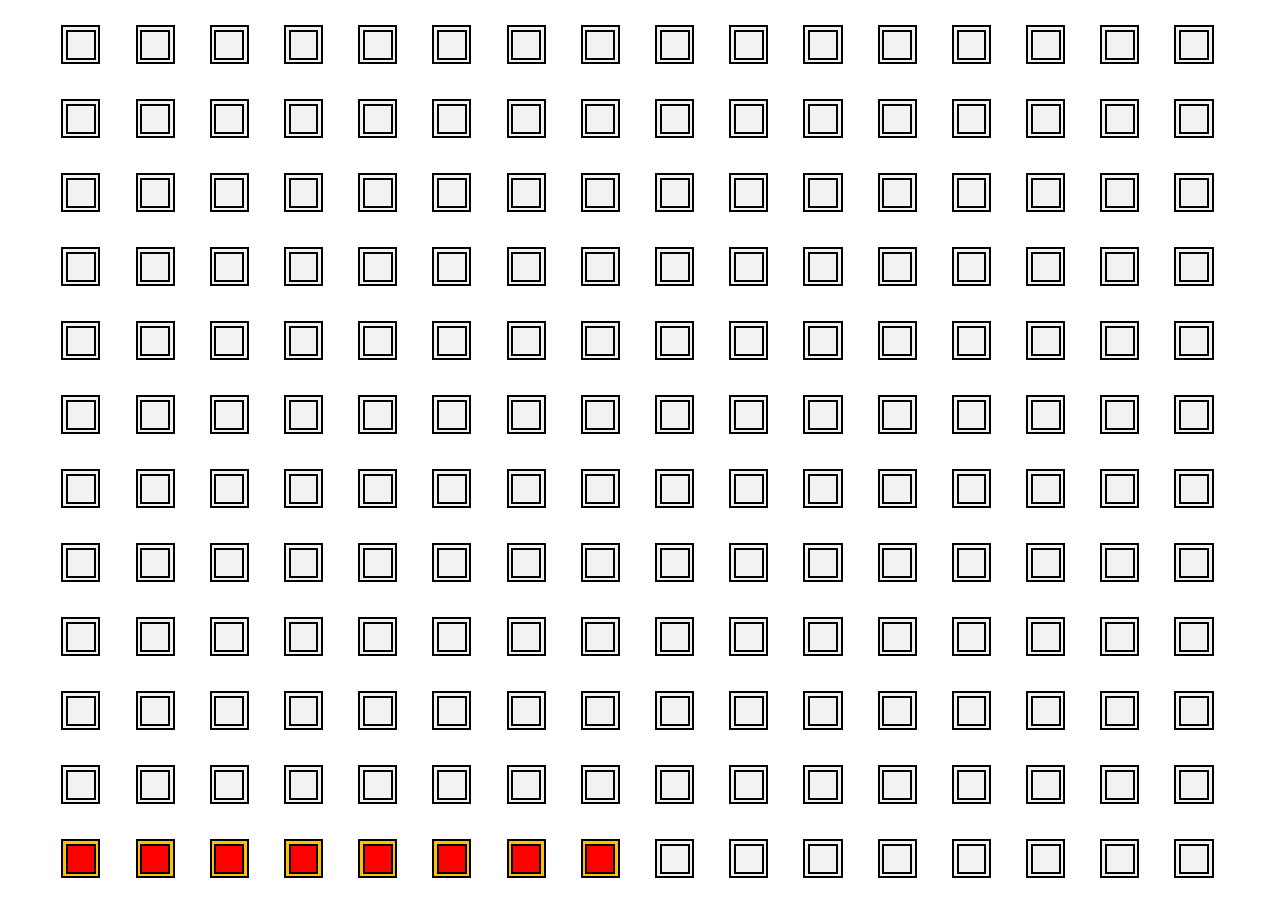
\includegraphics[width=0.35\linewidth]{figs/fig4.8.pdf}
    \caption{Серые элементы антенной решетки отключены во время оценки угла прихода на CSI-RS}
    \label{fig:4.8}
\end{figure}
>>>>>>> main
\subsection{Оценка мощности}

Поскольку разрабатываемые алгоритмы должны быть основаны на мощности, ключевым
моментом является способ измерения мощности сигнала. Для каждой пары лучей UE-BS
у нас есть набор пилотных поднесущих, поэтому есть два пути измерения:
\begin{enumerate}
    \item Усреднить мощность по всем пилотным поднесущим.
    \item Использовать Фурье преобразование по всем пилотным поднесущим, перейти
    от частотной характеристики канала к временной и оценить мощность как
    максимум импульсной характеристиках канала.
\end{enumerate}

Возьмем для начала однолучевую модель канала. В этом случае сигнал, принятый на $q$-ой пилотной поднесущей примет вид
\begin{equation}
    x_q = a e^{-i2\pi q\Delta f \tau} + \xi_q,
\end{equation}
где $a$ комплексная амплитуда луча, включающая в себя диаграмму направленность
элемента, $\Delta f$ расстояние между пилотными поднесущими в частотной области,
$\tau$ -- задержка распространения, $\xi$ -- комплексны белый гауссовый шум с
мощностью $\sigma^2$.
Для первого варианта, оцененная мощность примет вид
\begin{equation}
    \hat p_1 = \frac{1}{Q} \sum\limits_{q = 0}^{Q - 1} \abs{x_q}^2,
\end{equation}
где $Q$ -- число пилотных поднесущих. После несложных вычислений, можем получить
\begin{equation}
    \mean{\hat p_1} = \abs{a}^2 + \sigma^2.
\end{equation}
\begin{equation}
    D_1 = \mean{p_1^2} - \mean{p_1}^2 = \frac{1}{Q}\qty(2\abs{a}^2 \sigma^2 + \sigma^4),
\end{equation}
где $\mean{\dots}$ -- математическое ожидание, $D$ -- дисперсия оценки мощности.



Во всех алгоритмах нас интересует $\abs{a}^2$ или пропорциональная ей величина.
Относительная систематическая ошибка $\delta_{s1}$ и относительная случайная ошибка $\delta_{r1}$ равны
\begin{equation}
    \delta_{s1} = \frac{\mean{\hat p_1} - \abs{a}^2}{\abs{a}^2} = \frac{\sigma^2}{\abs{a}^2},
\end{equation}
\begin{equation}
    \delta_{r1} = \frac{\sqrt{D_1}}{\abs{a}^2} =
    \frac{1}{\sqrt{Q}} \sqrt{2 \frac{\sigma^2}{\abs{2}} +
        \frac{\sigma^4}{\abs{a}^4}},
\end{equation}
Для второго варианта, оцененная мощность будет вычисляться следующим образом
\begin{equation}
    \hat p^2 = \max_n\qty(\frac{1}{Q} \sum\limits_{q=0}^{Q-1} x_q e^{-2 \pi q n /Q})^2,
\end{equation}
где $n$ -- индекс в оцененной дискретной ИХ канала. 
Если предположить, что выбор максимума всегда осуществляется корректно, можно
получить следующее
\begin{equation}
    \mean{\hat p_2} = \abs{a}^2 F + \frac{1}{Q}\sigma^2.
\end{equation}
\begin{equation}
    D_2 = \mean{\hat p_2^2} - \mean{\hat p_2}^2 = \frac{2\abs{a}^2 F \sigma^2}{Q},
\end{equation}
\begin{equation}
    F = \max_n \frac{\sin^2[\pi Q (\Delta f \tau - n/Q)]}{Q^2 \sin^2[\pi(\Delta f \tau - n/Q)]},
\end{equation}
\begin{equation}
    \frac{4}{\pi^2} \leq \frac{1}{Q^2 \sin^2[\frac{\pi}{2Q}]} \leq F \leq 1,
\end{equation}


\hl{
Таким образом, мы видим, что оценка мощности тоже смещена, но систематическая
ошибка меньше, чем в первом случае.
Так как любой постоянный коэффициент $F$ не важен в алгоритмах}, а
лишь обеспечивает дополнительный выигрыш во временной области, относительную
систематическую ошибку $\delta_{s2}$ и относительную случайную ошибку $\delta_{r2}$ следует
определять как
\begin{equation}
    \delta_{s2} = \frac{\mean{\hat p_2} - F \abs{a}^2}{F \abs{a}^2} = \frac{1}{Q} \frac{\sigma^2}{F\abs{a}^2},
\end{equation}
\begin{equation}
    \delta_{r2} = \frac{\sqrt{D_1}}{F\abs{a}^2} = \frac{1}{\sqrt Q} \sqrt{\frac{2\sigma^2}{F\abs{a}^2}}.
\end{equation}

\hl{
Если мы используем только пилотные поднесущие для оценки мощности и $FQ > 1$ (т.е. $Q\geq 3$),
мы можем гарантировать, что $\delta_{s2} \leq \delta{s1}$. Поэтому, второй подход к оценке дает меньшую
систематическую ошибку. Что касается случайной ошибки, мы можем сказать, что $\delta_{r_2} \leq \delta_{r_1}$, если
$\abs{^2}/\sigma^2 < 0.34$ (т.е. SNR на поднесущую составляет -4.7 дБ или меньше).
}

Таким образом, второй подход к оценке мощности для моноимпульса (см. \ref{sec:monopulse}) и случаев с
низкими ОСШ. Также, если задачей является оценка направления на основной луч в
многолучевом канале, второй подход уменьшает помехи, вызванными остальными лучами.
Однако в случае многолучевой оценки угла прихода второй подход приводит к
большой сложности, из-за необходимости рассматривать трехмерную задачу для
каждого возможного пути распространения.

Таким образом, в работе применяются следующая схема оценки мощности
\begin{enumerate}
    \item Для оценки угловой координаты в многолучевом канале, используется первый подход (усреднение принятой мощности по пилотным поднесущим) \\
    \item Для оценки угловой координаты в однолучевом канале, применяется второй подход (Time Of Arrival selection) \\
\end{enumerate}
